\documentclass[UTF8,nofonts,cs4size]{ctexrep}
\setCJKmainfont{AR PL SungtiL GB} %中文为wqy 微米黑字体
%插入c代码使用的包,及其设定
\usepackage{color}
\usepackage{listings}
\lstset{language=C}%这条命令可以让LaTeX排版时将C++键字突出显示
\lstset{breaklines}%这条命令可以让LaTeX自动将长的代码行换行排版
\lstset{extendedchars=false}%这一条命令可以解决代码跨页时,章节标题,页眉等汉字不显示的问题

\lstset{
  language=C,
  keywordstyle=\color{blue},
  numbers=left,
  basicstyle=\ttfamily,
  frame=leftline,
  breaklines=true,
%  texcl=true,
%  backgroundcolor=\color{green!69!yellow!30!}
}

% 设定页边距
\usepackage[top=2.5cm,bottom=2.5cm,left=2.5cm,right=2.5cm]{ geometry}
% 加载 ams 数学公式与数学字体宏包
\usepackage{amsmath, amsfonts}
\usepackage{graphicx}
%设置首行缩进
\usepackage{indentfirst}
\setlength{\parindent}{2em }
\setlength{\parskip}{0pt }
%段前段后距离设置
\CTEXsetup[beforeskip=0ex]{paragraph}
%页眉和页脚
\usepackage{fancyhdr}
\pagestyle{fancy}
\lhead{}
\chead{}
\rhead{}
\lfoot{}
\cfoot{\thepage}
\rfoot{}
\pagenumbering{Roman}

\begin{document}
%设置中文章节的格式的字体
\CTEXsetup[format={\centering\zihao{3}}]{chapter}
\CTEXsetup[format={\bf\zihao{4}}]{section}
\CTEXsetup[format={\bf\zihao{-4}}]{subsection}

%设置中文摘要
\CTEXoptions[abstractname={\zihao{3}摘要}]
\begin{abstract}

NIM游戏又叫拈游戏或者"尼姆"游戏。传说来自于中国。这种游戏的一般玩法是将许多石子分成任意列数,每列中有
任意枚数石子(大于零)。然后两位玩家轮流取子,直至一方无子可取认输为止。本文阐述了NIM游戏的起源和一
般玩法。并介绍了几种常见的NIM游戏的变形游戏及其玩法。比如:威氏游戏、简单的单堆游戏、奇偶游戏、随机单
堆游戏、双倍游戏。在此基础上探讨了该类游戏的制胜策略及其数学原理。该类游戏存在必胜策略,即使用判断是否为安
全组合的方法。而NIM游戏通过将每列中石子个数用二进制表示法表示,然后对某一局面所有列中的石子个数进行异或运
算来判断该局面是否为安全组合。而威氏游戏则将某一局面中所有石子个数用斐波那契数列表示法表示,通过判断个数较小
的一列通过补零左移是否能够得到另外一列石子个数,而判断该局面是否是安全组合。并且使用归纳法等证明方法,证明
了其数学原理。在了解了NIM游戏的玩法和数学原理基础上,使用c语言实现了NIM游戏的一种玩法。
\paragraph{}
关键字:NIM游戏、变形玩法、异或运算、表示法、补零左移、c语言实现
\end{abstract}
%设置外文摘要
\CTEXoptions[abstractname={\zihao{3}ABSTRACT}]
\begin{abstract}
\indent \ \ NIM twist game was  also called "Nim" game. It's was said coming from China. This game is played with a lot of stones generally be divided into any number of columns, each column in any number of pieces of stones (greater than zero). Then two players take turns to take children up to one free throw in the towel until the child desirable. This paper describes the origin and general NIM game play. And introduces several common distortion NIM game and play the game. For example: Wei's game, the simple single-stack game, parity games, randomized, single pile game, double game. On the basis of a winning strategy for such games and mathematical principles. The existence of such a winning strategy game, that is as safe to use to determine whether the combination of methods. The NIM game by the number of stones in each column in binary notation, and then all the columns of a situation were different in the number of stones or shipped Calculation to determine whether the security situation in combination. And Wei's game will be all the stones of a number of situations with Fibonacci series notation, by judging by the number of the smaller one is left zero padding can be also a number of stones, and judge the situation whether it is safe combination. And the use of induction and other proof to prove that Its mathematical principles. NIM in the understanding of mathematical principles and the rule of the game, based on the NIM using C language game of play. 
\paragraph{}
Keywords: NIM game, deformation play, XOR, representation, left zeros, c language


%设置目录的格式
\CTEXoptions[contentsname={\zihao{3}目\ 录}]
\tableofcontents



\end{abstract}
\pagenumbering{arabic}
\chapter*{前言}
\addcontentsline{toc}{chapter}{前言}
NIM游戏是一个流传于民间的古老而富有趣味的游戏。因为它的游戏道具选取方便,所以成为了人们茶余饭后休闲益智的一种常见的游戏。本文从游戏的取胜策略的角度,研究这种游戏的规则及其各种形式的变形游戏的规则。虽然这些游戏的制胜策略也各有差异,但其理论本质可以归结为数学原理。本课题旨在在探寻这类游戏及其各种变形的玩法规则和制胜策略的基础上,对广泛传播于大众间的NIM游戏能够进行计算机模拟,实现人机对弈。
\paragraph{}
\indent \ \ 
关于NIM游戏的制胜策略,在很长的一段时间内,人们都没有找到。玩游戏的人只是凭借着自己的经验和运气来玩这个游戏。而且关于NIM游戏的的现有文献资料并不是很丰富,能查到的绝大多数文献资料都是关于Charles L. Bouton博士的一篇论文《Nim,A Game with a Complete Mathematical Theory》的一些进一步阐述。Bouton博士的这篇论文提出了一种简单易行的方法,来赢取游戏的胜利。这也改变了人们以往只能凭借着运气和经验来赢取比赛的局面。Bouton博士的这种方法是基于一种不进位的二进制加法来实现的。这种二进制加法的表述是这样的:二进制表述的数对应的位相加的时候,结果产生的进位舍弃。通过这种计算Bouton博士将游戏的当前状态分成安全组合和不安全组合。安全组合是指二进制加法结果的各个数位上的数皆为偶数,即2或者0。虽然这种计算方法在手算的时候,很简便。但是计算机实现起来却略显麻烦。通过观察和测试,我将这种计算方法替换为了异或运算。其结果还是一样的。
\paragraph{}
\indent \ \ 
在Bouton博士研究出一般的NIM游戏的制胜策略的时候。同时,也揭示了这个游戏在游戏一开始的时候就能判断出游戏的输赢。也就是说,这个游戏是一个可以预知输赢的游戏。这样一来,我们就进一步研究了游戏玩家在玩这个游戏的时候输与赢的各自的概率。
\paragraph{}
\indent \ \ 
对于一般意义上NIM游戏的研究完成后,又研究了一下NIM游戏的变形及其玩法。关于这方面的文献资料并不是很多,本论文中所涉及的各种玩法的规则皆来自于网络。NIM游戏的变形游戏的变异方法可以大致分成这样几类。第一种是改变游戏的取胜规则,即最后无子可取的人胜。第二种是改变游戏过程的规则。比如双倍游戏中规定,每位玩家所能取走的石子数量的最大值为上一次玩家所取走的石子数量的两倍。在这里我们介绍了以下集中NIM游戏的变形及其玩法:威氏游戏、单堆游戏、奇偶游戏、双倍游戏、随机单堆游戏。并对他们的规则和一般玩法进行了阐述。同时研究了其中几种的制胜策略。这里主要是指威氏游戏。
\paragraph{}
\indent \ \ 
对于威氏游戏制胜策略的研究是仿照bouton博士的方法进行的。Bouton博士的方法关键部分,除了对游戏当前状态的分类外。还有就是对于使用了二进制表示法来表示石子数量,进行状态判定。于是我尝试使用相同的方法,来研究威氏游戏的制胜策略。但是发现二进制表示法,在威氏游戏中失效了。在参考了一些关于数制表示法的文献资料后,发现使用斐波那契表示法,可以很好的解决这个问题。即如果游戏当前状态中数值较大的一列是通过数值较小的一列在斐波那契表示法下左移一位得到的,那么这种状态就是安全组合。
\paragraph{}
\indent \ \ 
最后,在研究了NIM游戏及其变形的基础之上。我使用c语言实现了一般的NIM游戏的人机对弈程序。在论文中阐述了主要的设计思路和实现方法。


\chapter{NIM游戏简介}
\section{NIM游戏的起源和游戏规则}
NIM游戏又叫拈游戏或者“尼姆”游戏。在所有的双人对弈游戏中,这个游戏是极其古老且富有兴趣的一个。据说拈游戏起源于中国古老的取火柴棍游戏“翻摊”,“翻摊”是一句广东话,又叫“拧法”。游戏时有数堆火柴棍,每堆有若干火柴棍,双方轮流从其中一堆取走一至若干根火柴棍,这样谁取到最后一根算输。“翻摊”游戏传到国外后非常流行,先是传到了被贩卖到美洲的奴工们手中。 称之为NIM(中文译音为“尼姆”),大概取音“拧法”而来。那里辛苦的工人们,在工作闲暇之余,用石头玩游戏以排遣寂寞。之后流传到上层社会中,人们用辨士(Pennils),在酒吧柜台上玩。这个传播的过程中,NIM游戏产生了许多变种。从游戏的胜负判定原因上改变,这种游戏通常双方轮流走子,走到最后,谁无子可走即赢得游戏。不像通常意义上的NIM游戏,无子可取即认输。或者直接从游戏过程中的规则改变游戏,产生了单堆游戏、威氏游戏等。虽然他们所使用的道具不尽相同,但是游戏规则也不尽相同,但是他们却都是NIM游戏的变种。虽然NIM游戏和它的变形游戏规则看似简单,玩起来也不是很困难,但是这种游戏中却蕴含了非常深奥的数学道理。
\paragraph{}
\indent\ \ 
而且Nim游戏也是博弈论中最经典的模型之一,它又有着十分简单的规则和无比优美的结论。同时Nim游戏也是组合游戏(Combinatorial Games)的一种,准确来说,属于“Impartial Combinatorial Games”(以下简称ICG)。一般意义上满足以下条件的游戏是ICG:
\\ \indent 1、有两名选手;
\\ \indent 2、两名选手交替对游戏进行移动(move),每次一步,选手可以在(一般而言)有限的合法移动集合中任选一种进行移动;
\\ \indent 3、对于游戏的任何一种可能的局面,合法的移动集合只取决于这个局面本身,不取决于轮到哪名选手操作、以前的任何操作、骰子的点数或者其它什么因素;
\\ \indent 4、如果轮到某名选手移动,且这个局面的合法的移动集合为空(也就是说此时无法进行移动),则这名选手负。
\\ 根据这个定义,很多日常的游戏并非ICG。例如象棋就不满足条件3,因为红方只能移动红子,黑方只能移动黑子,合法的移动集合取决于轮到哪名选手操作。而NIM游戏的规则则很像然满足这个ICG的特点。一个具有代表性的NIM游戏规则表述如下:
\newline
\indent
1、有两名选手;
\newline
\indent 2、两名选手交替对游戏进行移动(move),一次一步,选手可以在(一般而言)有限的合法移动集合中任选一种进行移动;
\newline
\indent
3、对于游戏的任何一种可能的局面,合法的移动集合只取决于这个局面本身,不取决于轮到哪名选手操作、以前的任何操作、骰子的点数或者其它什么因素;
\newline
\indent
 4、如果轮到某名选手移动,且这个局面的合法的移动集合为空(也就是说此时无法进行移动),则这名选手负。
\section{NIM游戏的一般玩法}
在上面的一节中,介绍了一般的NIM游戏的规则。其实,游戏规则规定了这个游戏应该以怎样的方式玩。但是由于游戏初始状态的不同,也就会有千千玩玩中玩法。而图\ref{example} 演示了一个常见的NIM游戏(三四五游戏)的过程。游戏的规则就像上面所讲的一样。假设刚开始有三堆石子$(x,y,z)$,每堆石子的石子个数分别为:3,4,5。有两名选手A、B。下面A先取石子。
\begin{figure}[htp]
\centering
\[ \begin{tabular}{cccc}
x & y & z & 策略 \\
3 & 4 & 5 & A从x堆中取走2个石子 \\
1 & 4 & 5 & B从z堆中取走3个石子 \\
1 & 4 & 2 & A从y堆中取走1个石子 \\
1 & 3 & 2 & B从y堆中取走1个石子 \\
1 & 2 & 2 & A从x堆中取走1个石子 \\
0 & 2 & 2 & B从y堆中取走1个石子 \\
0 & 1 & 2 & A从z堆中取走1个石子 \\
0 & 1 & 1 & B从y堆中取走1个石子 \\
0 & 0 & 1 & A从z堆中取走1个石子 \\
0 & 0 & 0 & A获胜,B惨败 \\
\end{tabular}  \]
\caption{三四五游戏}
\label{example}
\end{figure}
 我们展示的这个游戏过程,只是三四五游戏千千万万中可能的玩法的其中的一种。在游戏的过程中,游戏者A和B都会对当前的石子状态进行判断,并根据当前的石子状态来选择出他们关于下一次取子的策略。在这个游戏过程中经过几轮的角逐,A最终获得了胜利。而B因为最后无子可取输掉了游戏。
\paragraph{}
\indent\ \
如果这个游戏只是(三、四、五)型态,那么不久后,大部份人就能熟悉其中规律,并且变得没有兴趣。 有一个改变的方法是,将铜板的列数增加,一一列的枚数改变。 这样的做法,的确使人有毫无规律的感觉,至少不至于像(三、四、五)型态的拈一样易于把握。而随着游戏规模的改变游戏变得复杂起来,人们便开始寻找这种游戏的制胜策略。然而在很长一段时间内,人们只能通过经验和运气来玩这个游戏。并没有一个很好的方法能够使游戏玩家来预测游戏的走向和选择能够使自己获得游戏最终的胜利的策略。
\paragraph{}
\indent\ \
直到本世纪初,哈佛大学数学系副教授查理士·理昂纳德·包顿(Chales Leonard Bouton) 提出一篇极详尽的分析和证明$^{\cite{bouton}}$,利用数的二进位表示法,解答了这个游戏的一般法则:对任意列数的石子,一列有任意枚数,什么样的策略才是致胜策略。
\paragraph{}
\indent\ \
在包顿的论文中,他阐明了在玩家$A$一次取子后所造成的当前石子状态,不是安全组合就是不安全组合。当当前局面是安全组合的时候,无论当前选手选择怎样的策略取子,都不能使局面到达另外一个安全组合。也就是如果对方,在以后的游戏过程中不出现什么错误的话,这名游戏玩家就会输掉这场比赛。而当当前局面是不安全组合的时候,当前的游戏玩家总是能够通过采取适当的策略将石子状态转移到一个安全组合。这样在以后游戏过程中,只要他不出现什么失误的话,他将会赢的这场比赛。
\paragraph{}
\indent\ \
包顿博士用来判断当前局面是否为安全组合的方法很简单。首先将各堆石子的枚数化成二进制表示,然后将他们按照数位对齐,并将相应的数位相加。如果结果的各个位都是偶数(为0或者能够被2整除),那么就说明这个局面是个安全组合;否则,如果有一位是奇数,则为不安全组合。而通过仔细的研究可以很容易发现,其实包顿博士的这种加法所得到的结果,与我们很熟悉的异或运算所产生的结果一模一样。但是异或运算在电脑上实现起来比较方便,在论文以后的阐述中。我们不使用包顿博士的无进位二进制加法,而是用异或运算进行阐述这个制胜方法的数学原理。下面举个例子来说明什么是安全组合
例如\{3,4,5\}游戏,一开始就是不安全组合。
\begin{equation}
011\oplus 100 \oplus 101 = 010
\end{equation}
\indent
先取子的人可以通过拿去适当的石子令石子状态转移到某个安全组合,比如从第一列中取走2枚,形成\{1,4,5\}
样的局面。
\begin{equation}
010\oplus 000 \oplus 010 = 000
\end{equation}
\indent
按照包顿博士的方法,这个游戏是有必胜策略的。就是说,在游戏一开始的时候就注定了谁将会赢得游戏的胜利。当然这个是建立在游戏双方都熟悉包顿博士的这个理论并且在他们的整个游戏过程中没有失误的前提下。比如,游戏一开始就是安全组合,那么这名游戏玩家,因为无法将石子状态转移到另外的某个安全组合而最终将会输掉比赛。游戏一开始是不安全组合,那么这名玩家就可以通过在适当的堆中取走适当枚数的石子而将石子状态转移到一个安全状态并最终赢得游戏胜利。当游戏双方都了解了包顿博士的方法之后,输赢就只能靠游戏刚开始的时候随机的产生的状态是否对自己有利了。

\chapter{NIM游戏的变形及其玩法}
用来玩NIM游戏的道具不限于石子。石头可以玩;无聊磕瓜子时,瓜子可以玩;围棋子可以玩……虽然各种各样的道具在变幻着,但这些都不是重点。改变游戏的道具当然也就能够形成NIM游戏的一些变形,比如擦线游戏。但是游戏的玩法却始终遵循着一般NIM游戏的玩法。NIM游戏的变形游戏一般改变的是游戏的输赢判定方法和游戏过程中的规则。对于改变游戏的输赢判定方法,我们可以将一种NIM游戏或者她的变形游戏中规定输赢的标准变成,最后无子可取的游戏玩家取的游戏胜利。对于这样的变形玩法,和原始游戏的玩法大同小异。游戏者只需要对换一下在一般NIM游戏中的思路就能够找到制胜策略。我们真正关心的是改变游戏过程中的规则的变形游戏。我们可以改变游戏中石子的堆数和石子堆数的状态,我们可以改变取子的规则。而且在游戏的过程中我们还可以用一些类似于骰子和纸牌一样的辅助道具。于是各种各样真正有意思的NIM游戏的变形就这样产生了。下面就介绍一下几种常见从NIM游戏演变而来的游戏及其玩法。当然在这里我们所讨论的玩法并非是指那种只能够通过经验和运气来玩游戏的方法,我们是指那种可以使玩家获得游戏胜利的方法。
\section{威氏游戏(Wythoff's Game)}
将拈的规定略加修改,成为只有两列的威氏游戏,却非常有意思。更改后的规定表述如下:游戏在开始的时候只有两堆,每一堆中有任意枚数的石子,两位玩家轮流取石子,玩家在取子的时候的游戏规则是,该玩家可以在任一列中取一枚或多枚石子,或者同时在两列取同样枚数的石子,玩家至少要取走一枚石子,直到最后将石子取光的人赢。当然也可以像一般的NIM游戏一样在判定游戏输赢的时候有相反的规定,判定最后将石子取光的人输。但在这里我们更关心游戏取子规则改变而产生的变形游戏。在这里只讨论前者。
\paragraph{}
\indent\ \
在这里一般的NIM游戏的玩法(包顿博士的理论)完全不能适用于威氏游戏。所有拈的安全组合$\{n, n \}$,在威氏游戏中都是不安全组合。 因为我们在游戏的取子规则中加了一个规定,游戏玩家可以从两列石子中同时取相同枚数的石子。
\paragraph{}
\indent\ \
例如:[例1]若n是正整数,则\{0,n\}和\{n,n\}都是不安全组合。
\paragraph{}
\indent\ \
[例2]而\{1,2\}是安全组合。因为他的一一种取子后的状态都是不安全组合。如图\ref{1122}。
\begin{figure}[htp]
\centering
\begin{align}
&\{1,2\}\overset{\mbox{从第二列取走1枚}}{\longrightarrow}\{1,1\} \notag \\
&\{1,2\}\overset{\mbox{从第二列取走2枚}}{\longrightarrow}\{1,0\} \notag \\
&\{1,2\}\overset{\mbox{从第一列取走1枚}}{\longrightarrow}\{0,2\} \notag \\
&\{1,2\}\overset{\mbox{从第一、二列各取1枚}}{\longrightarrow}\{0,1\}  \notag 
\end{align}
\caption{(1,2)之后所有可能的策略}
\label{1122}
\end{figure}
不管采取哪种取子策略产生的局面都是不安全组合。
\paragraph{}
\indent \ \ 
[例3]\{3,5\}是安全组合,因为无论对方取何种策略,总会达到例1的不安全组合,而你总是可以通过适当的侧罗,造成例2的安全组合。所以\{3,5\}是安全组合。如图\ref{3355}所示。
\begin{figure}[htp]
\centering
\begin{align}
&\{3,5\}\overset{\mbox{每列各取1枚}}{\longrightarrow}\{2,4\}\overset{\mbox{第二列取3枚}}{\longrightarrow}\{2,1\}  \notag \\
&\{3,5\}\overset{\mbox{每列各取2枚}}{\longrightarrow}\{1,3\}\overset{\mbox{第二列取1枚}}{\longrightarrow}\{1,2\}  \notag \\
&\{3,5\}\overset{\mbox{每列各取3枚}}{\longrightarrow}\{0,2\}  \notag \\
&\{3,5\}\overset{\mbox{第一列取1枚}}{\longrightarrow}\{2,5\}\overset{\mbox{第二列取4枚}}{\longrightarrow}\{2,1\}  \notag \\
&\{3,5\}\overset{\mbox{第一列取2枚}}{\longrightarrow}\{2,5\}\overset{\mbox{第二列取3枚}}{\longrightarrow}\{1,2\}  \notag \\
&\{3,5\}\overset{\mbox{第一列取3枚}}{\longrightarrow}\{0,5\}  \notag \\
&\{3,5\}\overset{\mbox{第二列取1枚}}{\longrightarrow}\{3,4\}\overset{\mbox{每列取2枚}}{\longrightarrow}\{1,2\}  \notag \\
&\{3,5\}\overset{\mbox{第二列取2枚}}{\longrightarrow}\{3,3\}  \notag \\
&\{3,5\}\overset{\mbox{第二列取3枚}}{\longrightarrow}\{3,2\}\overset{\mbox{各列取1枚}}{\longrightarrow}\{2,1\}  \notag \\
&\{3,5\}\overset{\mbox{第二列取4枚}}{\longrightarrow}\{3,1\}\overset{\mbox{第一列取1枚}}{\longrightarrow}\{2,1\}  \notag \\
&\{3,5\}\overset{\mbox{第二列取5枚}}{\longrightarrow}\{3,0\} \notag 
\end{align}
\caption{(3,5)之后所有可能的策略}
\label{3355}
\end{figure}

\paragraph{}
\indent\ \
如果照这样的逻辑推演下去,可以得到很多安全组合\{1,2\},\{3,5\},\{4,7\},\{6,10\}……
通过观察很容易看出第n组安全组合$\{a_n,b_n\}$有以下定义:
\\ \indent\ \ (1)$a_1=1,b_1=2$
\\ \indent\ \ (2)如果$a_1,b_1.....a_{n-1},b_{n-1}$已经得到,那么$a_n$为上面$2n-2$个数中未出现过的
最小整数。
\\ \indent\ \ (3)$b_n=a_n+n$
\paragraph{}
\indent\ \
如果将上面所提到的种种组合表示出来就像图\ref{safe}所示。
\newline
\begin{figure}[htp]
\centering
\begin{tabular}{|c|c|c|c|c|c|c|c|c|c|c|}
\hline n & 1 & 2 & 3 & 4 & 5 & 6 & 7 & 8 & 9 & ..... \\
\hline $a_n$ & 1 & 3 & 4 & 6 & 8 & 9 & 11 & 12 & 14 & ..... \\
\hline $b_n$ & 2 & 5 & 7 & 10 & 13 & 15 & 18 & 20 & 23 & ..... \\
\hline
\end{tabular}
\caption{安全组合}
\label{safe}
\end{figure}
\paragraph{}
\indent\ \
这个时候我们就找到了一种类似于包顿博士的方法,获得了威氏游戏的制胜策略。但是,这种方法还有欠缺。没有使用优美的数学语言来阐述这种方法背后的数学原理。这个工作我们将在后面的章节中进行。但是此时,只要熟记上面的图中的安全组合,一个游戏玩家就可以在这种威氏游戏中取得比较好的成绩。
\section{单堆游戏}
\subsection{简单的单堆游戏}
在所有一般的NIM游戏的的变形游戏中,单堆游戏是比较简单的一种。他的游戏规则从一般NIM游戏改变而来。不但改变了游戏的堆数,而且改变了游戏的取子规则。最常见并且为大众所熟悉的玩法是这样的:在一个单堆游戏开始的时候,只有一堆石子,石子的数量是任意给定的。两位游戏玩家轮流取子,各人各次最少取1个,最多取k个,最后取光石头的人赢得此游戏。游戏在取子规则上改变了以往一般NIM游戏在取子的时候没有上限的规定,使用一个随机确定的数k来表示每次游戏玩家所能够取子的上限。
\paragraph{}
\indent\ \
和前面的情况一样。我们仍然使用当前状态判定的方法来探讨这种游戏的制胜策略。该游戏的所有局面可以分成两种情况:安全组合和不安全组合。而在单堆游戏中$k+1$扮演着极其重要的角色。因为每次一个玩家所能取走的石子个数$i$,有$1\leq i < k+1$。于是
\[
1 \leq k+1-i \leq k
\]
而另外一个玩家在遵守规则的情况下总是可以取走$k+1-i$个石子,使得这两次总共取走$k+1$个石子。于是可见$k+1$是安全组合。利用归纳法也容易得到有$k+1$的整数倍的石子个数的局面也是安全组合反之,不是$k+1$倍数的任意自然数$n=q(k+1)+r$,其中$1 \leq r \leq k$。一次拿r个石子就能够达到安全组合$q(k+1)$,可见此时为不安全组合。知道了当前局面是否为安全组合,玩家就可以根据当前局面,通过适当的策略达到最终胜利。
\subsection{奇偶游戏}
奇偶游戏是单堆游戏中较复杂的一种。他的规则表述如下:两个人轮流取一堆石子,各个人各次最少取走1个,最多取走k个,到最后石子被去逛时,若手中所有石子总数为奇数,则此人赢得游戏(也可以规定,当手中石子总数为偶数时赢得游戏)。

\subsection{随机单堆游戏}
当在单堆游戏中引入传统的游戏工具骰子时,便产生了随机单堆游戏。该游戏的规则表述如下:有一堆数目不定的石子。由一位玩家任意掷一枚骰子,开出现几点,就取去几枚石子。而后两位玩家轮流翻转骰子到前一次骰子出现的那一面旁边的四个面中的任意一个面,但不可以翻到对面,也不可以不翻,翻到几点就取去几枚石子。如此轮流,直到一方没有办法继续取石子为止。此时这位玩家就输了。
\paragraph{}
\indent\ \
随机单堆游戏和简单单堆游戏有点相似,但却不同。如果骰子出现i的时候轮到你取子。则从1到6中的个数有两个,即i和7-i你不能够翻到。你只能翻到其余四个面。所以各次你能够取去的石子个数,受制于对手所翻到的数目而定。而对手所能翻到的数目也受制于你翻到的数目。如此相互影响。游戏就变得复杂而不可捉摸。但是在游戏过程中按照简单单堆游戏的安全组合的判断方法,依然可以在适当的情况下给自己制造安全组合。
\subsection{双倍游戏}
双倍游戏和随机单堆游戏有一个共同特征,就是各次所取去的石子个数受到上次对方所拿石子个数的影响。一般双倍游戏的规则表述如下:两位玩家轮流取子,各个人各次最少取走一枚石子,最多取走上次对方所拿石子个数的两倍;最后拿光石子的人赢得此次游戏。并且第一位玩家不能取走全部的石子。
而且我们通过推演可以得到下面的结论:
\newline
[例4]1是安全组合。因为对方没有合适的策略可以取子。
\newline
[例5]2是安全组合。因为对方只能取走一枚石子。
\newline
[例6]3是安全组合。因为
\[3\overset{\mbox{对手取1}}{\longrightarrow}2 \overset{\mbox{你取2}}{\longrightarrow}0 \ \ \ \ \ 3\overset{\mbox{对手取2}}{\longrightarrow}1 \overset{\mbox{你取1}}{\longrightarrow}0\]
如此推演下去,我们会发现所有斐波那契数列中的项都是双倍游戏的安全组合。而其余的自然数则是不安全组合。
\section{擦线游戏}
用来玩NIM游戏的道具不限于石子。石头可以玩;无聊磕瓜子时,瓜子可以玩;围棋子可以玩。当没有任何道具的时候,甚至数数也可以玩。这里我们介绍一种在缺少类似与石子这样的道具的时候的玩法——擦线游戏。这个游戏的玩法是:在一张纸上用笔做出任意线段数条,两人轮流用橡皮擦擦去若干相连的小段,如此轮流擦线,最后一个擦线而再无线段留下的人胜。这个游戏相对于一般的NIM游戏而言只是道具变成了我们信手可得的笔与橡皮。
\section{方形棋}
方形棋是NIM游戏的另外一种规定的变形玩法。他的规则乍看起来,可能与一般的NIM游戏迥异。这种游戏在游戏规则的改变上成都很大,但无论怎样改都保留了与数有关的一些规则。
\paragraph{}
\indent \ \ 
这个游戏的玩法表述如下:将16枚棋子(道具也可以是其他的)排成一个正方形,如图\ref{square}。

两位游戏玩家轮流从这个正方形中取棋子,取子的时候,可以在任意一列或者行中取一枚或者多枚棋子,但所取的棋子必须为同一直线上相连的棋子,直到最后无子可取的人输为止(当然我们也可以规定无子可取的人胜)。
\begin{figure}[htp]
\centering
\includegraphics[scale=1]{square.eps}
\caption{方形棋}
\label{square}
\end{figure}
\paragraph{}
\indent \ \ 
如果像然这个游戏变得更加复杂,那么可以增加正方形的边城,用五颗、六颗甚至更过的棋子来组成正方形的一条边。甚至可以改变这个游戏的棋子排成的形状。比如把棋子排成三角形,就变成了三角棋:将15枚棋子排列成三角形,如图\ref{angle}。两位玩家轮流从中拿去棋子,取子的时候,可以取一枚或者多枚棋子,但所取的棋子必须在一条直线上,最后将棋子取光的人赢得游戏。
\begin{figure}[htp]
\centering
\includegraphics[scale=1]{angle.eps}
\caption{三角棋}
\label{angle}
\end{figure}


\chapter{NIM制胜策略的数学原理}
\section{NIM游戏的制胜策略及其数学原理}
\subsection{制胜模型一}
假设我们不知道Buoton博士的方法,那么一般的NIM游戏看上去就有点复杂和不可琢磨。那么就先从简单情况开始研究吧。如果轮到你的时候,只剩下一堆石子,那么此时的必胜策略肯定是把这堆石子全部拿完一颗也不给对手剩,然后对手就输了。如果剩下两堆不相等的石子,必胜策略是通过取多的一堆的石子将两堆石子变得相等,以后如果对手在某一堆里拿若干颗,你就可以在另一堆中拿同样多的颗数,直至胜利。如果你面对的是两堆相等的石子,那么此时你是没有任何必胜策略的,反而对手可以遵循上面的策略保证必胜。如果是三堆石子……好像已经很难分析了,看来我们必须要借助一些其它好用的(最好是程式化的)分析方法了,或者说,我们最好能够设计出一种在有必胜策略时就能找到必胜策略的算法。
\paragraph*{}
\indent
\ \ 而且在玩NIM游戏的过程中,我们会发现可以将石子堆的当前状态分成两种状态:安全状态和不安全状态。一般对自己而言是安全状态的状态对对手而言就是不安全状态,对自己而言的不安全状态对对手而言就是安全状态。这里的安全状态和不安全状态指的是在这种状态下要取子的选手而言的。对于这两种状态的定义如下:
\newline
\indent
不安全状态: 当前没有石子可取的状态是不安全状态,所有移动都导致安全状态的是不安全状态。
\newline
\indent
安全状态:存在一种策略移动到不安全状态是安全状态。
\paragraph*{}
按照这个定义,如果局面不可能重现,或者说各个状态的集合可以进行拓扑排序,那么各个$stute$是安全状态还是不安全状态可以预先计算出来。下面举个例子来说明两种状态的具体含义。
\paragraph*{}
\indent
\ \ 很显然刚才演示过程中的$(0,0,0)$状态是不安全状态,因为当前没有石子可取是终结态。而$(0,2,2)$以后可能的各个状态用树形图来表示就如图\ref{change}所示。
\begin{figure}[ht]
\begin{center}
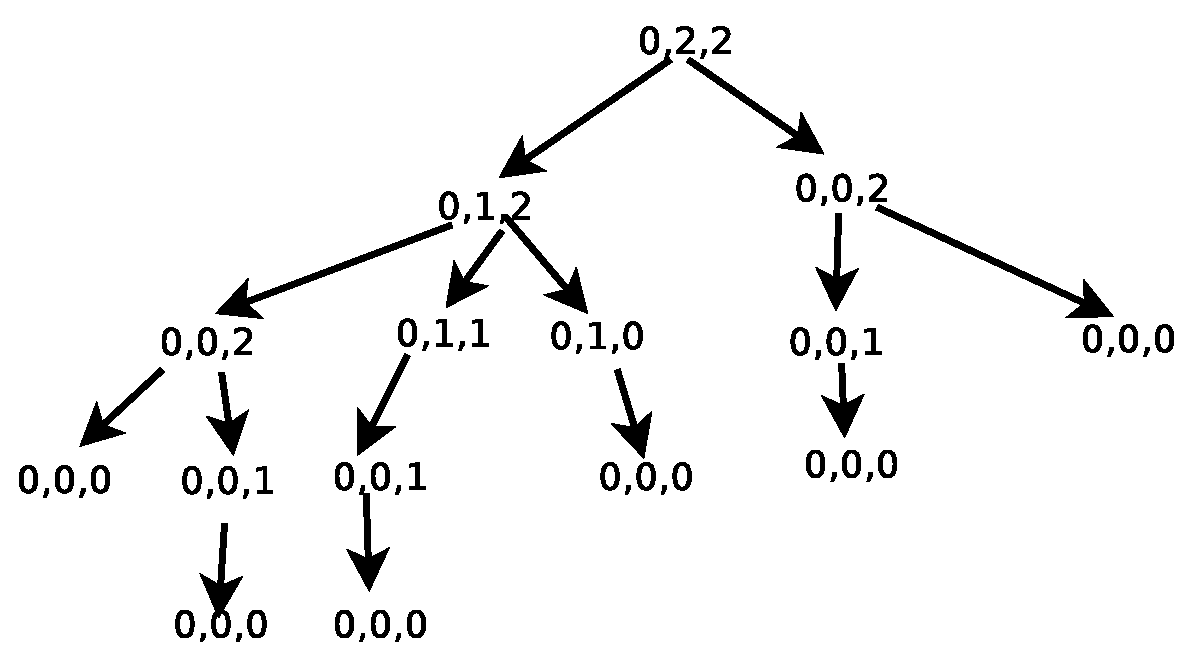
\includegraphics[scale=0.42]{dd.eps}
\end{center}
\caption{石子状态转移}
\label{change}
\end{figure}

%\newline 注:由于当两堆石子数目一样时,取石子的策略和取具体那一堆没有关系如当石子数目为(0,2,2)时,故略去一些相同策略
再上面的树形描述中根据定义很容易看出:$(0,0,0)$是不安全状态;于是$(0,0,2)$、$(0,1,1)、(0,0,1)$都是安全状态。因为$(0,1,1)$的唯一一种策略$(0,0,1)$是安全状态,所以$(0,1,1)$是不安全状态。于是$(0,1,2)$是安全状态。于是$(0,2,2)$的两种策略$(0,1,2)$,$(0,0,2)$都是安全状态。所以$(0,2,2)$是不安全状态。
\paragraph*{}
\indent\ \
根据上面这个过程,可以得到一个递归的算法——对于当前的局面,递归计算它的所有子局面的性质,如果存在某个子局面是不安全状态,那么向
这个子局面的移动就是可以令游戏玩家获得胜利的策略。这里存在大量的重叠子问题,所以可以用DP或者记忆化搜索的方法以提高效率。但问题是,利用这个算法,对于
某个Nim游戏的局面$(a_1,a_2,...,a_n)$来说,要想判断它的性质以及找出必胜策略,需要计算$O(a_1*a_2*...*a_n)$个局面的性质,不管怎样记忆化都无法
降低这个时间复杂度。所以我们需要更高效的判断Nim游戏的局面的性质的方法。这种方法使用计算机编程的方法来说很简单但是对于人类而言问题规模过于庞大。

\subsection{制胜模型二及其数学原理}
\paragraph{}
\indent\ \
在第一章中我们简单介绍了包顿博士提出了一种基于异或运算的解决办法。只要判断当前石子堆的状态是不是安全组合即可判断出这局游戏自己将会赢,还是将会输。而一种状态是安全组合,当且仅当该装态满足
\begin{align}
a_1 \oplus a_2  \oplus  ..... \oplus  a_n  = 0
\end{align}
为了证明上面的这个结论,需要证明以下三个命题。
\newline
\indent
1、所有最终状态$(0.....0)$判为安全组合;
\newline
\indent
2、被判为不安全组合的状态一定可以移动到某个安全组合;
\newline
\indent
3、被判为安全组合的状态无法移动到某个安全组合。

\indent
第一个命题显然,对于各一局NIM游戏来说最终状态只有一个,就是$(0....0)$。异或之后结果仍然是$0$。
\newline
\indent
第二个命题,对于某个局面$(a_1,a_2,...,a_n)$,若
\[a_1 \oplus a_2  \oplus  ..... \oplus  a_n  \neq 0\]
一定存在一个合法的移动在$a_i$变成$a_i^l$后满足:
\[a_1 \oplus a_2  \oplus  .. a_i^l... \oplus  a_n  = 0\]
不妨设

\[a_1 \oplus a_2  \oplus  ..... \oplus  a_n  = k\]
则一定存在某个$a_i$,他的二进制表示在k的最高位上是$1$。此时\[a_i \oplus k = 0\]一定成立。
则我们设\[a_i^l = a_i \oplus k\]
此时
\[a_1 \oplus a_2  \oplus  .. a_i^l... \oplus  a_n \oplus = a_1 \oplus a_2  \oplus  ..... \oplus  a_n \oplus k= 0\]

第三个命题,对于某个局面$(a_1,a_2,...,a_n)$,若
\[a_1 \oplus a_2  \oplus  ..... \oplus  a_n  = 0\]一定不存在一个合法的策略在$a_i$变成$a_i^l$后满足:
\[a_1 \oplus a_2  \oplus  .. a_i^l... \oplus  a_n  = 0\]。因为异或运算满足消去率,由
\[a_1 \oplus a_2  \oplus  .. a_i^l... \oplus  a_n \oplus = a_1 \oplus a_2  \oplus  ..a_i... \oplus  a_n = 0\]
得\[a_i=a_i^l\]。所以将$a_i$变成$a_i^l$不是一个合法的移动。
\newline 证毕。

\subsection{NIM游戏中的概率研究}
\indent
对于一局NIM游戏的参与者,而且在知道了上面的制胜模型之后,想要赢取此局游戏。除了尽量通过$xor$运算,给对手留下安全组合的状态之外,剩下的就是靠运气了。那么下面研究一下对于一局游戏开始时,一个游戏参与者将会赢的概率。
\paragraph*{}
\indent
\ \
在这个游戏中,一旦游戏刚开始的时候石子状态为不安全组合,取子者总可以通过适当的方法将安全组合留给对手。也就是说一旦第一个取子者在游戏开始就碰到了不安全组合,那么在接下来的游戏过程中,只要他不出差错,最终的赢家就是他。而第一个取子的玩家碰上安全组合时,在第二个玩家不出差错的情况下,最终的赢家将会是第二个取子的玩家。
\paragraph*{}
\indent
\ \
假设各个玩家都不会出错,并且各一堆石子的个数不超过$2^n$个,总共有3堆石子。并且各一堆石子在开始时都不会空。那么在开始时石子堆所能够呈现的状态
\begin{align}
Sum & =\frac{\binom{2^n-1}{1}\binom{2^n-2}{1}\binom{2^n-k}{1}}{k!}+\frac{\binom{3}{1}\binom{2^n-1}{1}\binom{2^n-2}{1}}{3}+\binom{2^n-1}{1} \notag \\
& =\frac{2^{n-1}(2^{2n}-1)}{3}
\end{align}
而刚开局就碰上安全组合的情况
\begin{align}
S^p & = \frac{(\binom{3}{0}+\binom{3}{2})^n-\binom{3}{1}\binom{2^n-1}{1}-1}{3!} \notag \\
& = \frac{(2^({n-1}-1)(2^n-1)}{3}
\end{align}
于是第二个取子者获胜的概率
\begin{align}
P(second) &= \frac{S^p}{Sum} \notag \\
&=\frac{\frac{(2^({n-1}-1)(2^n-1)}{3} }{\frac{2^{n-1}(2^{2n}-1)}{3}} \notag \\
&=\frac{2^{n-1}-1}{2^{n-1}(2^n+1)}
\end{align}
第一个取子者获胜的概率
\begin{align}
P(first) &=\frac{Sum-S^p}{sum} \notag \\
&=\frac{\frac{(2^({n-1}-1)(2^n-1)}{3}  -   \frac{(2^({n-1}-1)(2^n-1)}{3}  }{\frac{(2^({n-1}-1)(2^n-1)}{3} } \notag \\
&=\frac{2^{2n-1}+1}{2^{n-1}-1}
\end{align}

\section{威氏游戏的致胜策略及数学原理}
\subsection{威氏游戏的致胜策略}
在上面的讨论中我们得到了一个表可以用来简化威氏游戏的玩法,并且找到了一个简单
的致胜策略。但是该中方法需要记忆的东西繁多。于是我们希望想NIM游戏一样,找到
一种更加简便的方法。
\paragraph{}
\indent\ \
若果将威氏游戏中的各组安全组合用费氏数列标准表示法表示出来,如图\ref{wiff}。
\begin{figure}[htp]
\centering
$
\begin{array}{cccccccccccc}
n&\ &\ &a_n&\ &\ &\ &\ &b_n&\ &\ &\ \\
1&\ &\ &\ &\ &1&\ &\ &\ &1&0&\ \\
2&\ &\ &1&0&0&\ &\ &1&0&0&0 \\
3&\ &\ &1&0&1&\ &\ &1&0&1&0\\
4&\ &1&0&0&1&\ &1&0&0&1&0\\
5&1&0&0&0&0&1&0&0&0&0&0\\
6&1&0&0&0&1&1&0&0&0&1&0\\
7&1&0&1&0&0&1&0&1&0&0&0\\
8&1&0&1&0&1&1&0&1&0&1&0\\
\end{array}
$
\caption{威氏游戏中的各组安全组费氏数列标准表示法表示}
\label{wiff}
\end{figure}

仔细观察上面的表格可以发现$b_n$是经$a_n$左移一位得到的(补零移位)。
而且各个$a_n$最右边有偶数个连续的0。同时,很显然$b_n$最右边有
奇数个的0。这样我们要
检测一个局面$\{x,y\}(x<y)$是不是安全组合就可以将$x,y$化成斐波那契数列标准表示法
,再看看是否满足上述条件即可。这样一来我们便找到了一种简便的方法来判断一个局面
是否是安全组合,同时也可以通过适当的策略将一种局面转化成安全组合。
\subsection{威氏游戏致胜策略的数学原理}
上述$\{a_n,b_n\}$的性质只是通过观察得到的,下面将证明之。
\paragraph{}
\indent\ \
首先将自然数分成$A$和$B$两部分。$A$是所有斐波那契数列表示法中所表示的数
右边有偶数个连续0的自然数的集合;$B$是所有斐波那契数列表示法中所表示的数右边
有奇数个连续的0的自然数的集合。将$A$中所有的数从小到大排成数列$\{a_{n}^{'}\}_{n=1}^{\infty}$
。而$b_{n}^{'}$是$a_{n}^{'}$的斐波那契数列表示法中左移一位(补零移位)所得到的数。我们需要证明
\[
A=\{a_{n}^{'}|n\mbox{为自然数}\},B=\{b_{n}^{'}|n\mbox{为自然数}\}
\]
并且符合条件:
\newline
(1)数列$\{a_{n}^{'}\}_{n=1}^{\infty}$和$\{b_{n}^{'}\}_{n=1}^{\infty}$都是严格递增序列,有$b_{n}^{'}=a_{n}^{'}+n$
\newline
(2)$A\cup B = N, A\cap B = \emptyset $
条件(2)易于知道。我们只要证明$b_{n}^{'}=a_{n}^{'}+n$就可以了。于是分成下面两步证明。
\paragraph{}
\indent\ \
一、$b_{n}^{'}-a_{n}^{'}$,随着n增加而增加。也就是说,当$n>m$时,$b_{n}^{'}-a_{n}^{'}>b_{m}^{'}-a_{m}^{'}$
\paragraph{}
\indent\ \
证明:假设
\begin{eqnarray}
& a_{n}^{'} = l_r f_r+l_{r-1}f_{r-1}+\cdots +l_0f_0 \\
& b_{n}^{'} = l_r f_{r+1}+l_{r-1}f_{r}+\cdots +l_0f_1 \\
& a_{m}^{'} = l_{r}^{'}f_r+l_{r-1}^{'}f_{r-1}+\cdots +l_{0}^{'}f_0 \\
& b_{m}^{'} = l_{r}^{'}f_{r+1}+l_{r-1}^{'}f_{r}+\cdots +l_{0}^{'}f_0
\end{eqnarray}
上面均是斐波那契数列标准表示法。为了对齐公式$l_{r}^{'}$与$l_r$可能为0。因为数列$\{a_{n}^{'}\}_{n=1}^{\infty}$
严格单调递增,所以当$n>m$时,$a_{n}^{'}>a_{m}^{'}$。也就是说存在$s<r$,使得$l_i=l_{i}^{'}$对各一个$i>s$成立
$l_s>l_{s}^{'}$。同时因为:
\begin{eqnarray}
& b_{n}^{'} - a_{n}^{'} = l_r f_r+l_{r-1}f_{r-1}+\cdots +l_1f_1 + l_0 \\
& b_{m}^{'} - a_{m}^{'} = l_{r}^{'}f_{r}+l_{r-1}^{'}f_{r-1}+\cdots +l_{1}^{'}f_1+l_{0}^{'}
\end{eqnarray}
于是
\[
b_{n}^{'} - a_{n}^{'} > b_{m}^{'} - a_{m}^{'}
\]
\paragraph{}
\indent\ \
二、对于任意一自然数$x$,有一组$\{a_{n}^{'},b_{n}^{'} \}$使得$b_{n}^{'} =a_{n}^{'} + x$。
\paragraph{}
\indent\ \
证明:当$x$的斐波那契数列表示法右边有奇数个连续的0时,取$a_{n}^{'}=x0(f)$,$b_{n}^{'}=x00(f)$
。当$x$的斐波那契数列数列表示法有变有偶数个连续的0时,即
\begin{eqnarray}
x=l_{r}f_r+l_{r-1}f^{r-1}+\cdots  l_{2m}f_{2m},l_{2m}=1
\end{eqnarray}取
\begin{eqnarray}
& a_{n}^{'} = l_r f_{r+1}+l_{r-1}f_{r}+\cdots +l_{2m+1}f_{2m+2}+f_{2m}+f_{2m-2}+\cdots + f_0 \\
& b_{n}^{'} = l_r f_{r+2}+l_{r-1}f_{r+1}+\cdots +l_{2m+1}f_{2m+3}+f_{2m+1}+f_{2m-1}+\cdots + f_1
\end{eqnarray}
利用

\begin{align}
&(f_{2m+1}+f_{2m-1}+\cdots + f_1)-(f_{2m}+f_{2m-2}+\cdots + f_0) \notag \\
&=(f_{2m+2}-1)-(f_{2m}-1) \notag \\
&=f_{2m+2}-f_{2m+1}  \notag \\
&=f_{2m}
\end{align}
可得$b_{n}^{'} =a_{n}^{'} + x$成立。
\paragraph{}
\indent\ \
上面的证明不但证明了$\{a_{n},b_{n} \}$所具有的性质,而且说明了$b_n$的斐波那契数列表示法是通过$a_n$的斐波那契数列
表示法补零左移所得。而且通过(二)的证明,对于任意一个自然数x,不必再使用归纳法$a_1,b_1,a_2 \cdots $算起,一直算到
$a_x,b_x$。我们就可以直接算出$a_x$和$b_x$。不必再去记忆表中那些繁琐的数据。
\chapter{简单NIM游戏的实现}
\section{游戏实现分析及总体设计}
为了实现一个简单的人机对弈NIM游戏,可以使用模块化的设计方法,将游戏中涉及到的各个实体(石子,游戏者,等等)抽象成一个个模块。然后通过各个模块间的交互关系来涉及并实现游戏。通过观察第一章中所介绍的简单的NIM游戏的玩法。我们可以将所要实现的NIM人机对弈游戏描述如下:这个游戏有两个参与者。一个是人类玩家,另外一个机器玩家。由游戏的控制机构控制双方轮流取子,直至一方无子可取认输为止。而游戏的规则可以表述为,每一个玩家只能从任意一列中取走任意枚数的石子。可以看出一个人机对弈的NIM游戏主要有以下部分组成:机器策略生成,石子状态管理,游戏控制,交互界面和策略违规检测。
而每一部分完成的功能如下:
\\
\indent
机器策略生成:通过设定的游戏策略生成机制,生成游戏策略。以与人类游戏者完成对弈。
\\
\indent
石子状态管理:管理当前石子状态,接受由机器或者游戏者的策略,改变当前石子状态。
\\
\indent
游戏控制:决定当前由哪名选手取子。
\\
\indent
策略违规检测:检测人类游戏者的策略是否违反游戏规则。
\\
\indent
交互界面:显示当前的石子状态,并接受由人类玩家产生的策略。
\paragraph{}
并且各个模块间的交互关系如图\ref{module}所示。
\begin{figure}[htp]
\centering
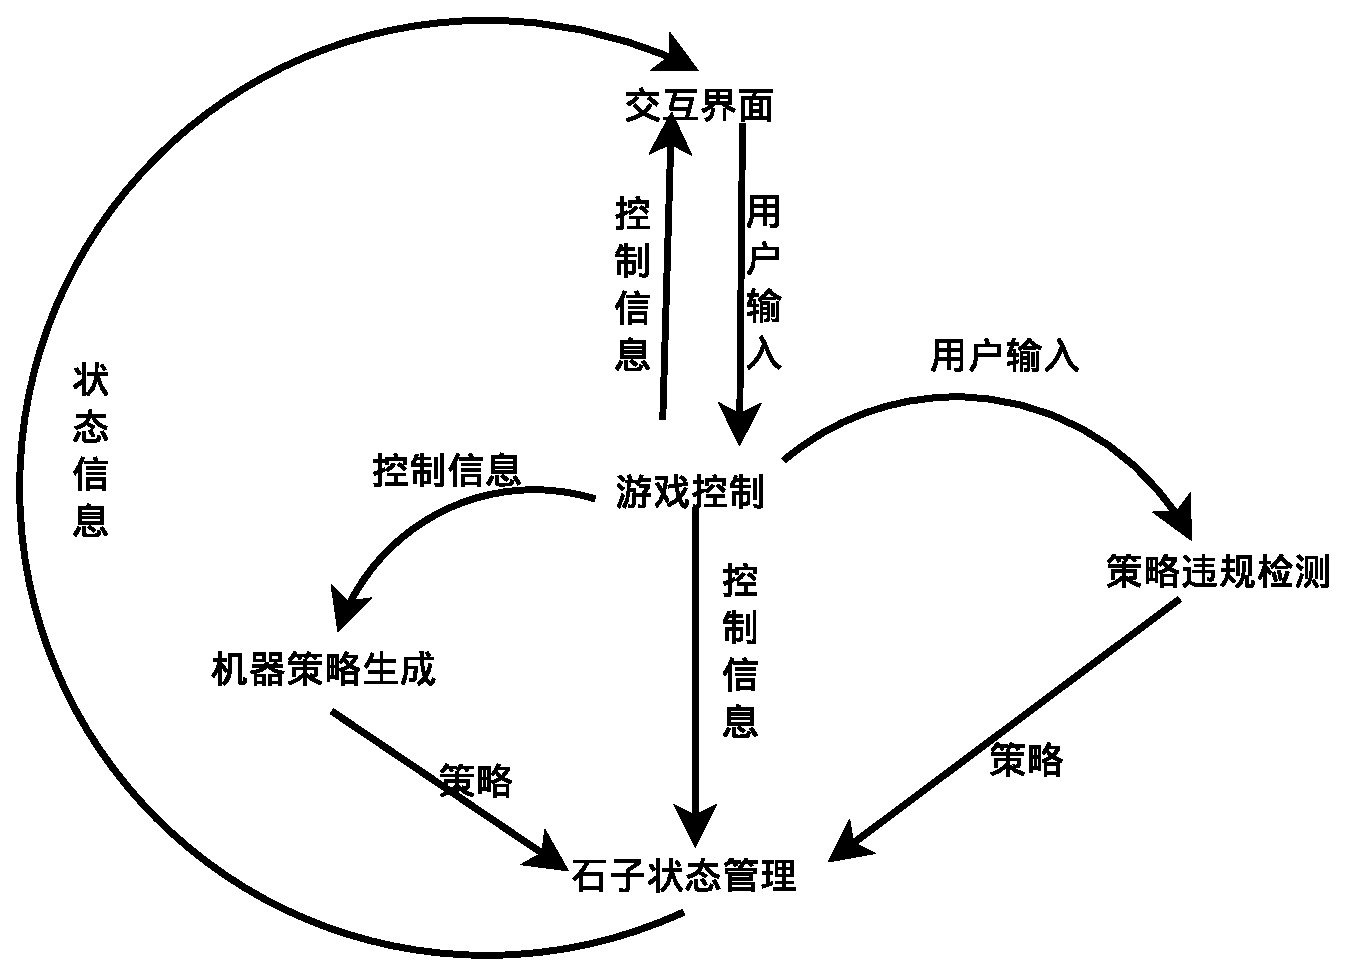
\includegraphics[scale=0.42]{Message.eps}
\caption{模块关系}
\label{module}
\end{figure}

\section{各模块的详细设计}
\subsection{石子状态管理模块}
观察整个游戏过程中的计数方法,会发现我们使用的是自然数计数法。所有的石子状态都是一系列自然数的组合。于是在程序中我们就可以用整形数组来表示石子当前状态。在程序中定义了两个关键的整形全局数组:Statue[TMAX]和change[TMAX]。前者指代当前石子的状态,而后者则是记录由机器玩家和经策略检测模块传递来的策略。并且,状态管理模块使用该策略改变Statue数组。这里TMAX预定义为10。当然游戏中石子的堆数并非只是10这个数。可能大于这个数,也可能小于这个数。当小于这个数时,数组的多余堆赋值为0;大于这个数的时候,数组动态扩展。于是该模块的主要功能就是监视Statue[TMAX]当前状态,并且将合适的change[TMAX]施加于Statue[TMAX]。
\subsection{交互界面模块}
游戏使用字符终端,玩家通过输入指令启动游戏。人类玩家可以控制石子总数,石子堆数,自己是否先手取子和游戏难度。而指令的格式如下:
\begin{lstlisting}
            Nim.exe [-S:[]] [-T:[]] [-H:[]] [-F/-NF]
            -S:[] : 总共石子数目。输入任意整数。
            -T:[] : 所要分的堆数。输入任意整数。
            -F    : 先手取子。
            -NF   : 后手取子。
            用法举例:
            linux平台下:./Nim -T:3 -S:10  -F
            windows平台下:Nim.exe -T:3 -S:10 -F
\end{lstlisting}
\indent
\ \
在玩家将游戏模型(石子总数,石子堆数,是否先手取子,游戏难度)确定下来后,游戏开始。当人类玩家取子时,玩家将依次输入该轮中对每一列石子所要释加的策略(若玩家不从某一列中取子,则对该列的策略为0)。
\paragraph{}
\ \
并且在一位玩家选择策略之后,游戏会通过字符显示的形式显示当前石子状态。
\subsection{游戏控制模块}
定义整形信号量first。当其为0时由人类玩家取子,其为1时由机器玩家取子。这个信号量的初值可由用户设定。
\subsection{机器游戏者模块}
该模块通过$Button$博士的理论,来产生游戏策略。其流程图如图\ref{celue}。
\begin{figure}[htp]
\centering
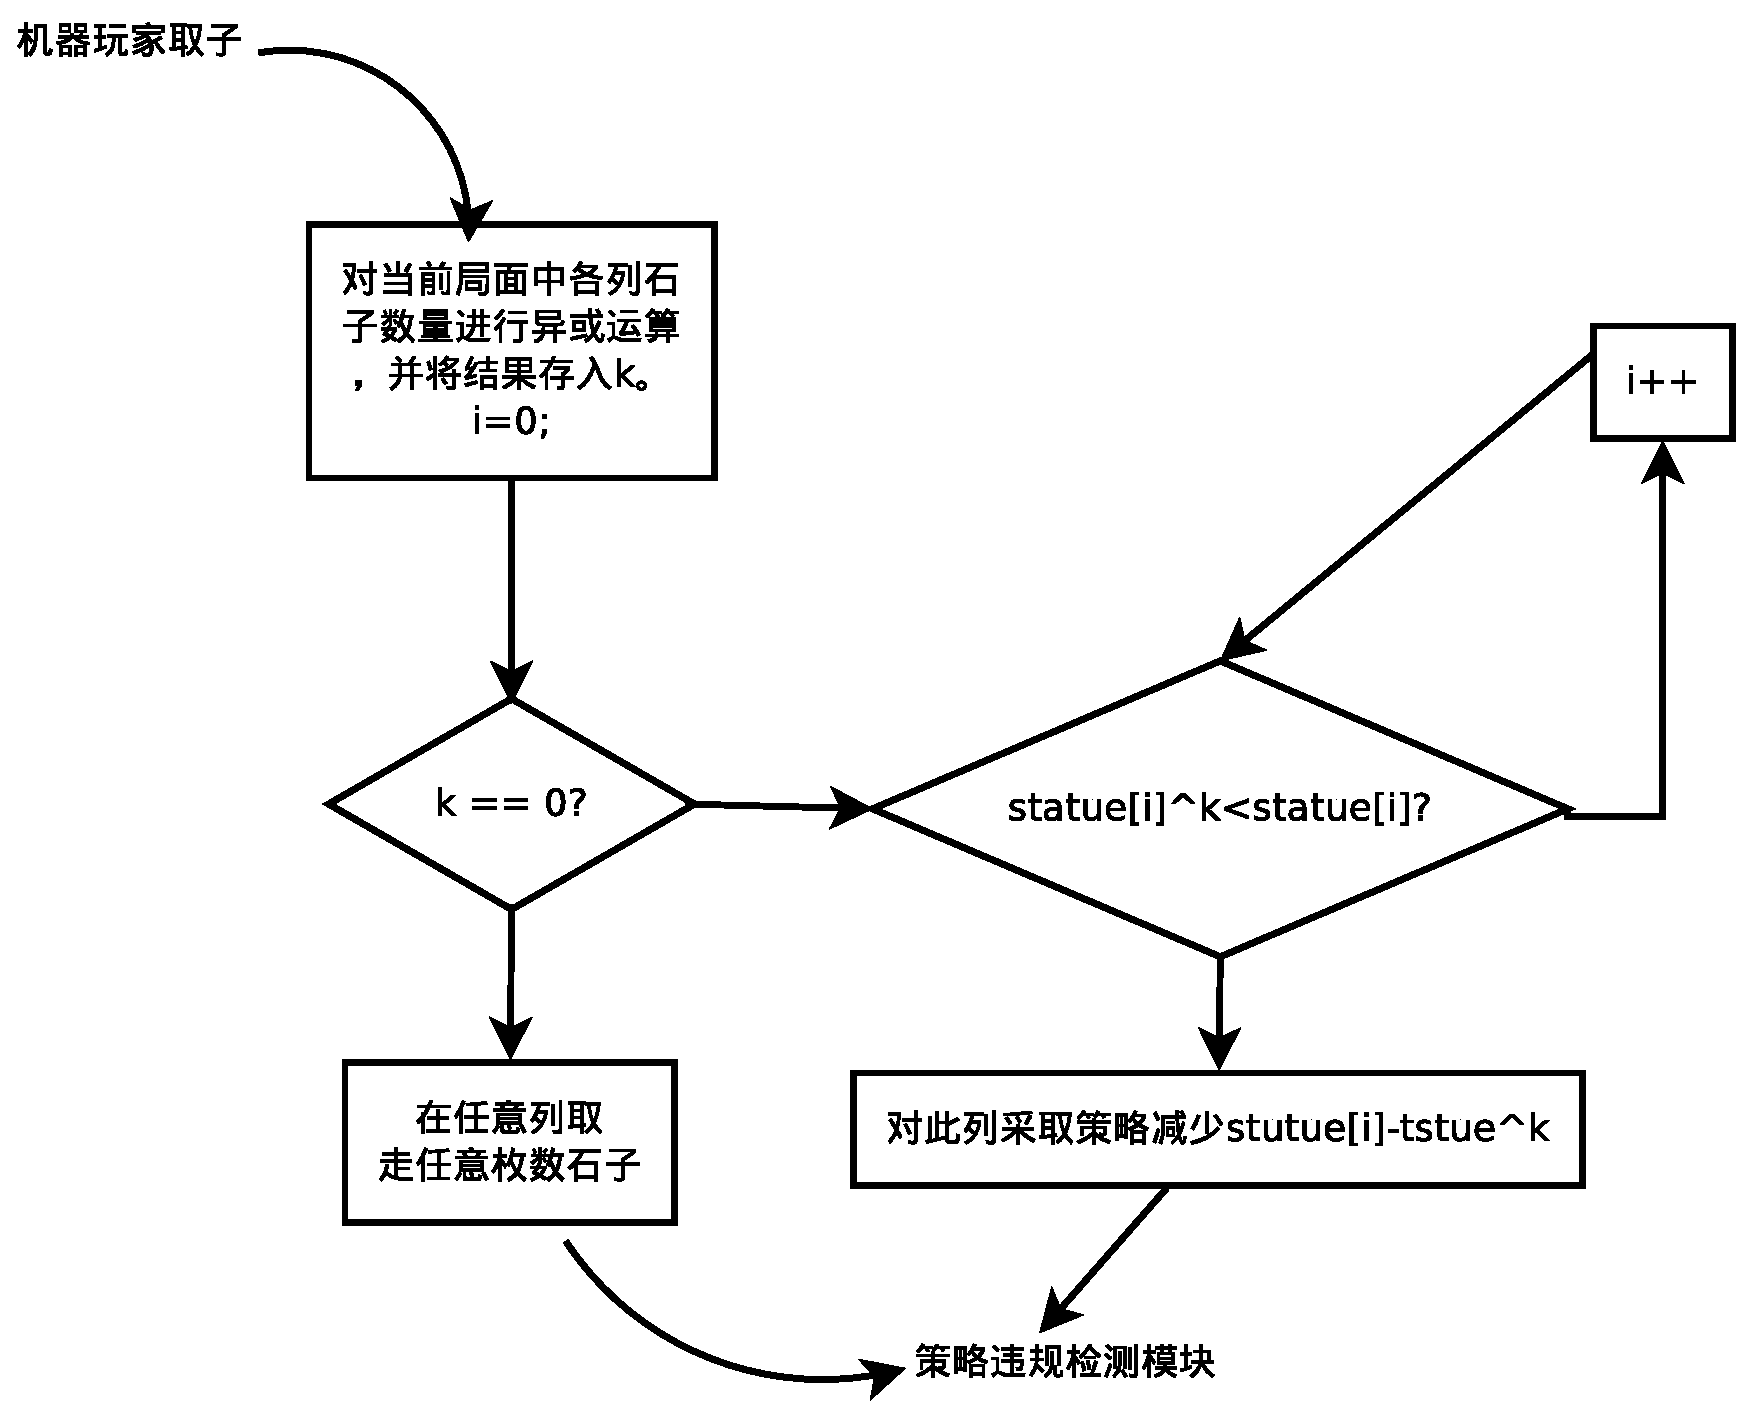
\includegraphics[scale=0.4]{celue.eps}
\caption{机器策略产生}
\label{celue}
\end{figure}
当当前局面是安全组合时,在任意一列中取走符合游戏规则的任意枚数石子。否则,使用$Button$博士的理论,来产生游戏策略。
\section{游戏演示}
在Ubuntu10.10环境下进行的一次游戏如图\ref{yunxing}所示。
\begin{figure}[htp]
\centering
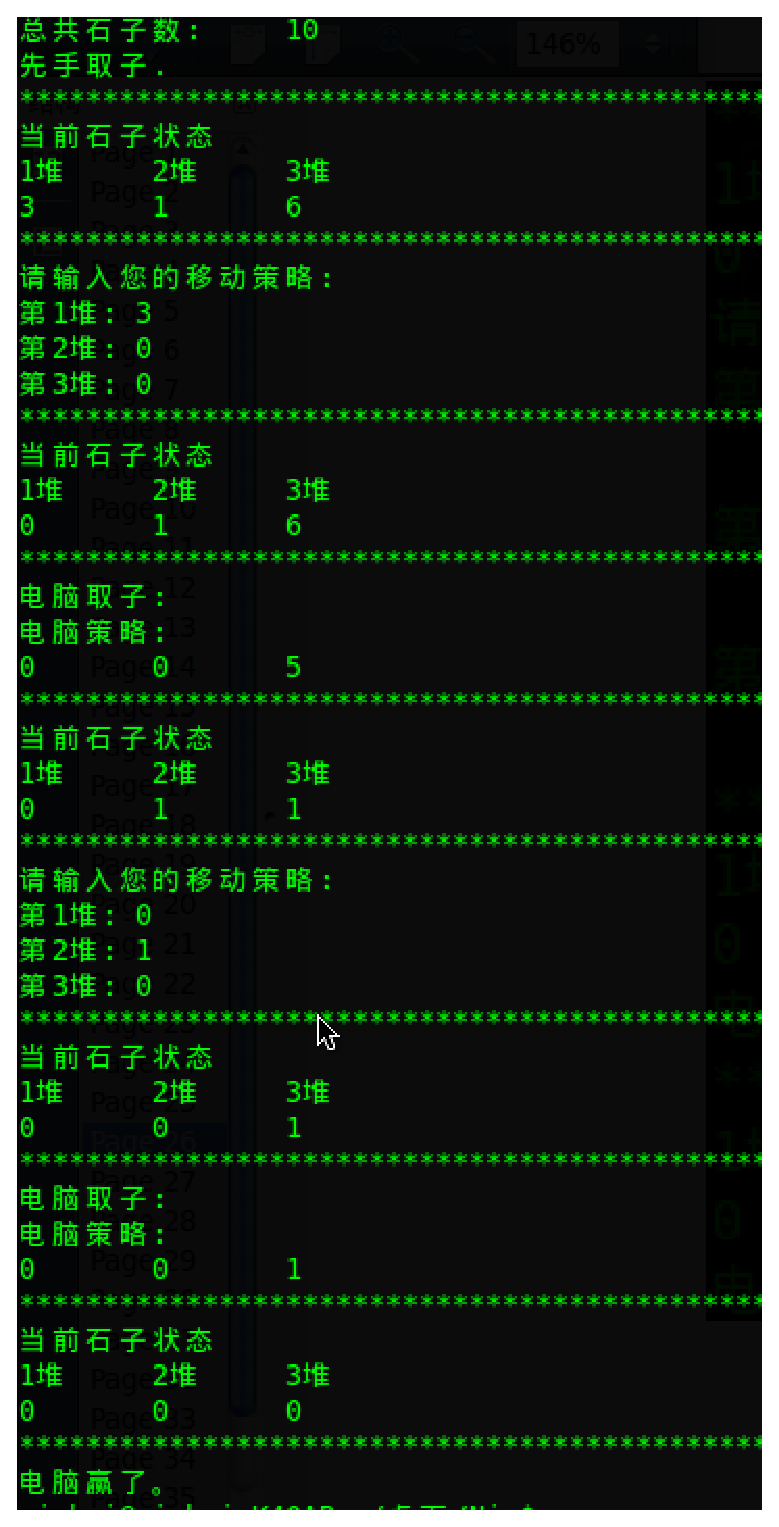
\includegraphics[scale=0.8]{002.eps}
\caption{游戏演示}
\label{yunxing}
\end{figure}
\chapter*{致谢}
\addcontentsline{toc}{chapter}{致谢}
光阴荏苒,日月如梭,在青岛理工大学的四年学习时间即将过去。在漫长的人生旅程中,三年时间并不算长,但对我而言,是磨砺青春、挥洒书生意气的三年,也是承受师恩、增长才干、提高学识的三年。我将以一个新青岛理工人的面貌,重新投入到火热的工作和事业中。在此,谨对培育我的母校、教导我的老师、帮助我的同学们致予最诚挚的谢意和敬意。 在此,我特别要感谢我的论文指导老师刘慧老师。刘慧老师,她学识渊博,专业精通,对青岛理工大学教育事业怀着深厚的感情;她诲人不倦,与同学们保持着良好的沟通并经常给予科学的指导和热心的勉励。就本篇毕业论文总结报告而言,从提纲、草拟、修改到最后定稿,刘慧老师都给予了一而再、再而三的精心批阅,每个环节都凝结老师努力的付出和辛劳的汗水。毋庸讳言,老师的为人处事将成为我人生的座标和里程碑。我还要感谢给予我很多关心和帮助的同学们,三年学习生活使我们结下深厚的友谊。俗话说天下没有不散之筵席,在毕业之际,我衷心地同学和朋友们在以后的人生道路上越走越宽广,也深深相信在未来的日子里我们将一路携手前行,会有很多的碰撞和交流,我们将始终记得我们曾在青岛理工大学同窗学习,这将是我克服困难、不断前进的精神动力。
\begin{thebibliography}{99}
\addcontentsline{toc}{chapter}{参考文献}
\bibitem{bouton}Charles L. Bouton.Nim,A Game with a Complete Mathematical Theory.The Annals of Mathematics, Second Series,Vol.3,No.1/4(1901-1907):35-39
\bibitem{computer}王晓东.计算机算法设计与分析.电子工业出版社,2007,138~178
\bibitem{youxi}A.M.Yaglom and I.M.Yaglom,《Challenging Mathematical Problems with Elementary Solutions》, vol.1 and 2,translated into English by James McCawley,Jr.
\bibitem{1}A.S. Fraenkel, Euclid and Wythoff games, Discrete Math. 304 (2005), 65–68.
\bibitem{2}M. Lothaire, Combinatorics on words, Cambridge Mathematical Library, Cambridge Univer-sity Press, Cambridge, (1997).
\bibitem{4}范如国.博弈论:武汉大学出版社,2011.
\bibitem{5}Bruldi,R.A祝,冯舜玺译.组合数学,北京:机系工业出版社,2005.
\bibitem{6}茆诗松,程依明,概率论与数理统计教程.北京:高等教育出版社,2004.
\bibitem{7}邵学才,叶秀明.离散数学.北京:电子工业出版社,2009

\end{thebibliography}
\appendix
\chapter{斐波那契数列表示法}
\section{数制表示法}
通常我们所用阿拉伯数字,即十进位表示法。是以$0,1,2,3,4,5,6,7,8,9$十个数字为基础,加以
借位的概念和“逢十进一”的方法组成。举个例子来说
\begin{equation}
    234=2*10^2 + 1*10 + 4 \notag
\end{equation}
而在文中我们所提到的二进制表示法,是由$0,1$两个数字为基础、借位的概念和“逢二进一”
的方法组成。举个例子来说:
\begin{equation}
    1010=1*2^3 + 0*2^2 +1*2^1+1*2^0 \notag
\end{equation}
在以上的例子中我们可以看到,各种进位法中,各个数位都是满足一定的数就会进位,比如:
十进制的“逢十进一”和二进制的“逢二进一”。
\paragraph{}
假设我们有一个自然数的无穷数列$B_0,B_1,B_2......$,其中$B_0=1$,其余各位均大于一。
这里假设我们有一种为B进位制的计数法则:从一个数的最右边开始算起,第一位满$B_1$进一
到第二位,第二位满$B_2$进一到第三位。以此类推。第$n$位满$B_n$,进一到第$n+1$位
于是,一个自然数$x$都会唯一的一个B进位表示法表示:$l_nl_n-1\dots l_1l_{0}B$。其中$0 \leq l_i \leq B_{i+1}$。于是
\begin{equation}
x=l_nl_n-1\dots l_1l_{0}B=\sum_{m=0}^{n}{l_mB_0B_1\dots B_m}
\end{equation}
在标准的十进制表示法中有$B_i=10, i =1,2\dots $。而二进制表示法中有$B_i=2,i =1,2\dots $.
\section{斐波那契数列表示法}
斐波那契数列是指无穷数列$1,1,2,3,5,8......$。他一般是通过递推公式
\begin{align}
&f_0=1,f_1=1  \notag \\
&f_n=f_{n-1}+f_{n-2}\ \ \ \ n\geq 2 \notag
\end{align}
求的。
而当以斐波那契数列为B进位制计数法的进位标准时(从$f_1$开始),就可以得到斐波那契数列表示法。即任何一个自然数$x$都可以用斐波那契数列表示法表述:
\[
x=\sum_{m=0}^{n}{l_mf_1f_2\dots f_m}
\]
比如自然数23用斐波那契数列表示法表示就是
\[
23=4*5+0*3+1*2+1
\]
\chapter{游戏源码}
\begin{lstlisting}
#include "stdio.h"
#include "string.h"
#include "stdlib.h"
#define TMAX 10
int Statue[TMAX];
int *StaPtr;
int change[TMAX];
int first = 0;

void init(int* a, int b)
{
	int i;
	for(i=0;i<b;i++)
		a[i] = 0;
}

void PrnStatue(int *statue, int tiples)
{
	int i;
	printf("******************************************************************\n");
	for(i=0;i<tiples;i++)
	{
		printf("%d堆\t",i+1);
	}
	printf("\n");
	for(i=0;i<tiples;i++)
	{
		printf("%d\t",statue[i]);
	}
	printf("\n");
}

void Increase(int* columm,int tiples)
{
	int temp[tiples];
	columm = temp;
}

void UsageMessage()
{
	printf("请在CMD下运行。用法错误,请按照一下格式使用:\n \\
Nim.exe [-S:[]] [-T:[]] [-H:[]] [-F/-NF] \n \\
-S:[] : 总共石子数目。输入任意整数。\n \\
-T:[] : 所要分的堆数。输入任意整数。\n \\
-H:[] : 游戏难度。1-10。难度递增。\n \\
-F    : 先手取子。\n \\
-NF   : 后手取子。\n \\
用法举例:\n \\
linux平台下:./Nim -T:3 -S:10 -H:1 -F\n \\
windows平台下:Nim.exe -T:3 -S:10 -H:1 -F\n");
}

void RandomTiple(int tiples , int sum)
{
	int i;
	int k;
	int random;
	if(tiples > TMAX)
	{
		Increase(Statue,tiples);
		init(Statue,tiples);
		Increase(change,tiples);
		init(change,tiples);
	}
	init(Statue,TMAX);
    for(i=0;i<tiples;i++)
	{
		if(i==tiples-1)
		{
			Statue[i]=sum;
			break;
		}
		{
			k = rand();
		//	printf("k=%d,sum=%d,random=%d\n",k,sum,k%(sum/2));
			random =k%(sum/2);
		}

//		for(;random > sum;random = 1);

//		printf("sumsss=%d\n",sum);
		sum = sum -random;
		Statue[i]=random;
	}
}


void ChangeStute(int* stute, int* change, int tiples)
{
	int i;
	for(i=0;i<tiples;i++) stute[i]=stute[i]-change[i];
}

int SumStone(int* stute, int tiples)
{
	int i,sum=0;
	for(i=0;i<tiples;i++) sum = sum +stute[i];
	return sum;
}

void PrnGuize()
{
	printf("请遵守游戏规则:每次只能移动一堆。\n");
}
void  SG(int* statue,int* change, int tiples)
{
	int i,k=0;
	init(change,tiples);
	for(i=0;i<tiples;i++)
	{
		k=statue[i]^k;
	}
	if(k!=0)
	for(i=0;i<tiples;i++)
	{
	 	if(((statue[i]^k)<statue[i]))
	 	{
	 	printf("statuei=%d,stautek=%d\n",statue[i],statue[i]^k);
	 	change[i]=statue[i] - statue[i]^k;
		printf("changei=%d\n",change[i]);
	 	return;
	 	}
	}

	for(i=0;i<tiples;i++)
	{
		if(statue[i] != 0)
		{
		change[i] = 1;
		return;
		}
	}

}


int TestChange(int *stute,int *change, int tiples)
{
	int i;
	int tempchange = 0;
	for(i=0;i<tiples;i++)
	{
		if(stute[i]-change[i] < 0) return 0;
		if(change[i] != 0)  tempchange++;
		if(tempchange>=2)  return 0;
	}
	if(tempchange = 0) return 0;
	return 1;
}


void BeginGame(int* stute, int* change, int tiples)
{
	int i;

	while(SumStone(stute,tiples) > 0)
	{
		if(first)
		{
			printf("请输入您的移动策略:\n");
			for(i=0;i<tiples;i++)
			{
				printf("第%d堆:",i+1);
				scanf("%d",&change[i]);
				printf("\n");
			}
			if(!TestChange(stute,change,tiples))
			{
				PrnGuize();
				continue;
			}
			ChangeStute(stute,change,tiples);
			if(SumStone(stute,tiples) > 0) first =0;
			PrnStatue(stute,tiples);
		}
		else
		{
			printf("电脑取子:\n");
			SG(stute,change,tiples);
			ChangeStute(stute,change,tiples);
			PrnStatue(stute,tiples);
			if(SumStone(stute,tiples) > 0) first =1;
		}
}
	if(first==1) printf("你赢了!\n");
	else printf("电脑赢了。\n");
}




int main(int argc,char** argv)
{
	int stone_sum = 20;
	int tiples = 3;
	int hard = 0;

	//辅助变量
	int i;
	char *temp;
	if(argc != 5)
	{
		UsageMessage();
		return 0;
	}

	/*命令筛选 */
	for(i=1;i<=argc-1;i++)
	{
		if(!strncmp("-T:",argv[i],3))
		{
			temp = strstr(argv[i],":");
			temp++;
			tiples = atoi(temp);
			printf("分成了:\t%d堆\n",tiples);
		}
		if(!strncmp("-S:",argv[i],3))
		{
			temp = strstr(argv[i],":");
			temp++;
			stone_sum = atoi(temp);
			printf("总共石子数:\t%d\n",stone_sum);
		}
		if(!strncmp("-H:",argv[i],3))
		{
			temp = strstr(argv[i],":");
			temp++;
			hard = atoi(temp);
			printf("难度系数为:\t%d\n",hard);
		}
		if(!strncmp("-F",argv[i],2))
		{
			first = 1;
			printf("先手取子.\n");
		}
		if(!strncmp("-NF",argv[i],3))
		{
			first = 0;
			printf("后手取子.\n");
		}
	}

	RandomTiple(tiples,stone_sum);
	PrnStatue(Statue,tiples);
	BeginGame(Statue,change,tiples);
	return 0;
}
\end{lstlisting}


\end{document}